\section{Policy-Hidden Outsourced ABE}

\begin{figure}
	\centering
	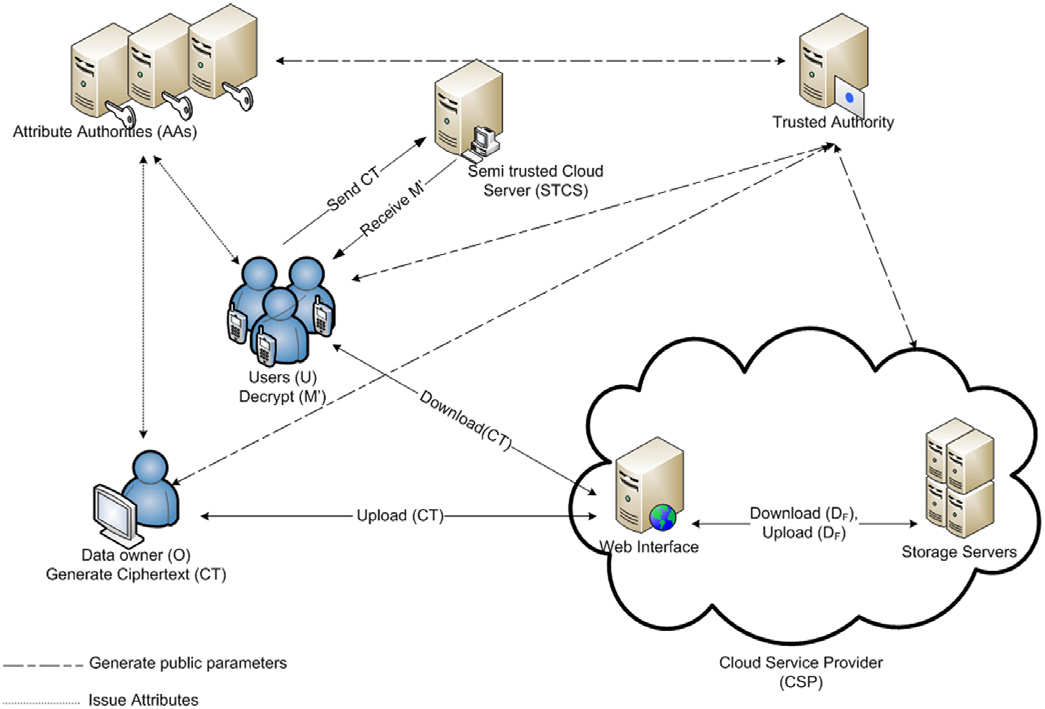
\includegraphics[width=0.8\textwidth]{phoabe-architecture}
	\caption{Architektur von PHOABE \cite{phoabe}}
\end{figure}

Es wird nun ein Überblick zu \textit{PHOABE} (Policy-Hidden Outsourced
Attribute Based Encryption) gegeben, einem Schema, welches aufgrund seiner
Architektur für attribut-basierte Verschlüsselung auf IoT-Geräten interessant
ist. Wie der Name bereits andeutet, handelt es sich hierbei um ein Schema,
welches die Geheimhaltung der Privatsphäre durch Zugriffsstrukturen
gewährleistet (Policy-Hidden). Zudem wird ein STCS verwendet, um den
Entschlüsselungsprozess teilweise auszulagern (Outsourced). Der Grund hierfür
ist, dass IoT-Geräte oft leistungsschwach sind und die Entschlüsselung
hingegen sehr kostspielig ist, weshalb viele andere ABE-Schemata nicht
praktikabel sind. Da ein STCS verwendet wird, stellt PHOABE zudem sicher, dass
die Integrität der Informationen gewährleistet ist. Der Grund für die
Sicherstellung ist, dass angenommen wird, dass der Server selbst korrupt sein
und versuchen könnte, private Daten auszuspähen, uns jedoch trotzdem valide
Ergebnisse erzeugt. Kurz zusammengefasst weist PHOABE folgende Eigenschaften
auf.

\FloatBarrier
\begin{itemize}
	\item Ausgelagert: Die Entschlüsselung wird teilweise durch einen Server
		(STCS) übernommen.
	\item Vertraulichkeit: Eine Änderung des Geheimtextes bewirkt keine
		sinnvolle Änderung der verschlüsselten Nachricht.
	\item Integrität: Es kann überprüft werden, ob die Resultate des STCS
		ge\-fälscht wurden.
	\item Geheimhaltung der Privatsphäre: Zugriffsstrukturen garantieren die
		Sicherung der Privatsphäre.
\end{itemize}

\subsection{Algorithmen}
PHOABE besteht aus insgesamt sieben Algorithmen \cite{phoabe}. Es werden
folgende Symbole für die Darstellung der Komponenten des Schemas verwendet.

\begin{enumerate}
	\item \algitem{Setup}{}{\lambda}{PP} Der
		Setup-Algorithmus nimmt als Eingabe einen Sicherheitsparameter $\lambda$,
		liefert die öffentlichen Parameter $\text{PP}$ und wird von einer
		\textit{Central Trusted Authority} (CTA) ausgeführt.
		\begin{enumerate}
			\item Definiere die multiplikativen Gruppen $\mathbb{G}_1$,
				$\mathbb{G}_T$ der Ordnung $p$.
			\item Definiere die bilinearen Abbildung $e: \mathbb{G}_1 \times
				\mathbb{G}_1 \to \mathbb{G}_T$.
			\item Setze den Generator $g$, sodass $\langle g \rangle = \mathbb{G}_1$.
			\item Definiere die Hashfunktion $H' : \left\{ 0,1 \right\}^* \to
				\mathbb{Z}_p$.
			\item Definiere die Hashfunktion $H_0 : \left\{ M \right\} \to \left\{ 0,1
				\right\}^{n_{H_0}}$. Die Ausgabe von $H_0$ besitzt dabei die feste Länge
				$n_{H_0}$.
			\item Definiere die Hashfunktion $H_1 : \left\{ M \right\} \to
				\left\{ 0,1 \right\}^*$.
			\item Definiere die Hashfunktion $H_2 : \left\{ 0,1 \right\}^* \to \left\{
				0,1 \right\}^{n_{H_2}}$. Die Ausgabe von $H_2$ besitzt dabei die feste
				Länge $n_{H_2}$.
			\item \textbf{return} $\left( \mathbb{G}_1, \mathbb{G}_T, p, H', H_0, H_1,
				H_2, e, g, e(g, g)\right)$.
		\end{enumerate}

	\item \algitem{Setup}{auth}{PP}{\left(sk_{AA_j}, pk_{AA_j}\right)} Bei $N$
		Autoritäten führt die Autorität $AA_j$ mit $j \in N$ diesen Algorithmus
		aus, um einen geheimen Schlüssel $sk_{AA_j}$ und einen öffentlichen
		Schlüssel $pk_{AA_j}$ zu generieren. Als Eingabe nimmt der Algorithmus die
		öffentlichen Umgebungsparameter $PP$. Im Folgenden sei die Menge der von der
		Attribute-Authority $AA_j$ bereitgestellten Attribute durch $S_{AA_j}$
		dargestellt.
		\begin{enumerate}
			\item Wähle zwei zufällige Zahlen $\alpha_i, t_i \in \mathbb{Z}^*_p$ für
				jedes Attribut $i \in S_{AA_j}$.
			\item Wähle eine zufällige Zahl $y \in \mathbb{Z}^*_p$.
			\item Setze den geheimen Schlüssel als $sk_{AA_j} = \left(
				\left\{\alpha_i, t_i \;\vert\; i \in S_{AA_j}\right\}, y \right)$.
			\item Berechne den öffentlichen Schlüssel \\
				$pk_{AA_j} = \left( \left\{ e(g, g)^{\alpha_i}, g^{t_i} \;\vert\; i \in
				S_{AA_j} \right\}, g^y \right)$.
			\item \textbf{return} $\left( sk_{AA_j}, pk_{AA_j} \right)$.
		\end{enumerate}

	\item \algitem{Encrypt}{}{PP, M_{pk}, m, \Phi}{C} Dieser Algorithmus
		ver\-schlüs\-selt die Nachricht $m$ unter Angabe einer Menge der
		öffent\-lich\-en Schlüssel $M_{pk} = \left\{ pk_{AA_j} \;\vert\; j \in N
			\right\}$ und wird vom Datenbesitzer ausgeführt. Jeder dieser Schlüssel
			werden von einer \textit{Attribute Authority} bereitgestellt. Zudem wird
			eine Zugriffsregel $\Phi = \left( A, \rho \right)$ verwendet. Als Ausgabe
			wird ein Geheimtext $C$ erzeugt.
		\begin{enumerate}
			\item Wähle eine zufällige Zahl $x \in \mathbb{Z}^*_p$
			\item Berechne für jedes Attribut $a_i$ den Wert $q_i = e((g^y)^x, H'(a_i))$,
				wobei $a_i \in \Phi$ ein Attribut aus der Zugriffsstruktur $\Phi$ ist
				und $\lvert\left\{a_i\right\}\rvert = F$.
			\item Konvertiere $\Phi$ mithilfe $\left\{q_i\right\}_{i \in F}$ in eine
				LSSS-Matrix $\left( A^{n \times l}, \rho \right)$, wobei $F$ die Anzahl
				der Attribute innerhalb der Zugriffsstruktur $\Phi$ ist. Die Umwandlung
				einer Zugriffsstruktur in eine LSSS-Matrix wird dabei als gegeben
				(Black-Box) angesehen.
			\item Wähle eine zufällige Zahl $s \in \mathbb{Z}_p$.
			\item Wähle $\left\{ p_i \;\vert\; p_i \in \mathbb{Z}^*_p \;,\; 0 \leq i < F
				\right\}$.
			\item Berechne $\lambda_i, \omega_i$ sodass $\lambda_i = \vec{A_i} \cdot
				\vec{v}$ und $\omega_i = \vec{A_i} \cdot \vec{\tau}$, wobei $\vec{v} =
				\left( s, v_2, ..., v_l \right) \in \mathbb{Z}^l_p$ und $\vec{\tau} =
				\left( 0, \tau_2, ... \tau_l \right) \in \mathbb{Z}^l_p$ zwei zufällige
				Vektoren aus dem $l$-dimensionalen Raum von $\mathbb{Z}_p$ sind. Die
				Verknüpfung zweier Vektoren mit $\cdot$ stellt dabei das Skalarprodukt
				dar.
			\item Berechne $CT_{ABE} = \left(h, C_0, C_{1,r}, C_{2,r}, C_{3,r}\right)$
				für jede Zeile $r$ aus der LSSS-Matrix $A$ mit
				$h = g^x$,
				$C_0 = R \cdot e(g, g)^s$,
				$C_{1,r} = g^{\lambda_{\rho(i)}} \cdot g^{\alpha_{\rho(i)}p_i}$,
				$C_{2,r} = g^{p_i}$ und 
				$C_{3,r} = g^{\omega_{\rho(i)}} \cdot g^{t_{\rho(i)}p_i}$.
				Zur Erinnerung: $\rho(i)$ gibt das Attribut $a$
				zurück, welches der Zeile $i$ der LSSS-Matrix zugeordnet wurde.
				Dementsprechend sind $\lambda_{\rho(i)}$ und $\omega_{\rho(i)}$
				zufällige Werte speziell für ein Attribut $a$.
			\item Wähle eine zufällige Nachricht $R \in \mathbb{G}_T$ aus der
				Zielgruppe und berechne $R_0 = H_0(R)$ und den symmetrischen Schlüssel
				$K_{sym} = H_1(R)$. Der Wert $R_0$ hat dabei eine beliebige während
				$K_{sym}$ eine feste Länge besitzt.
			\item Führe eine symmetrische Verschlüsselung der Nachricht $m$ durch,
				sodass $CT_{sym} = encrypt_{sym}\left(K_{sym}, m\right)$ und berechne den
				Verifizierungsschlüssel $V = H_2(R_0 || CT_{sym})$, wobei $||$ die Werte
				von $R_0$ und $CT_{sym}$ miteinander verkettet.
			\item \textbf{return} $C = \left(CT_{ABE}, CT_{sym}, V\right)$.
		\end{enumerate}

	\item\label{enum:phoabe_keygen} \algitem{Keygen}{}{PP, sk_{AA_j}, pk_{AA_j},
		GID, S_{j, GID}}{sk_{j, GID}} Dieser Algorithmus erzeugt einen privaten
		Schlüssel $sk_{j, GID}$ und wird von einer \textit{Attribute Authority}
		$AA_j$ ausgeführt. Der Schlüssel wird für einen Benutzer erzeugt und steht
		in Verbindung mit den Attributen $S_{j, GID} = \left\{ a_1, ..., a_{n_j}
		\right\}$ der $AA_j$.  Dabei stellt $a \in S_{j, GID}$ ein Attribut und
		$n_j$ die Anzahl der Attribute von $AA_j$ dar. $GID$ ist die Identität vom
		Benutzer.
		\begin{enumerate}
			\item Zur Erinnerung: $sk_{AA_j} = \left(\left\{\alpha_i, t_i\right\}_{i
				\in S_{AA_j}}, y\right)$.
			\item Berechne $K_{1,i} = g^{\alpha_i} \cdot H'(GID)^{t_i}$ für jedes
				Attribut $i \in S_{j, GID}$.
			\item Berechne $K_{2,i} = H'(i)^{y}$ für jedes Attribut $i \in S_{j,GID}$.
			\item \textbf{return} $sk_{j, GID} = \left\{ K_{1,i}, K_{2,i} \;\vert\; i \in S_{j,
					GID} \right\}$.
		\end{enumerate}

	\item \algitem{Transform}{}{PP, M_{sk}, (A, \rho), C}{T} Dieser Al\-go\-rith\-mus wird von einem Benutzer ausgeführt.
			Dieser besitzt eine Menge von Attributen $S_{GID}$ und die dazugehörigen
			Schlüssel $M_{sk} = \left\{ sk_{j, GID} \;\vert\; j \in N \right\}$ bei
			$N$ Attribute-Authorities. Die Schlüssel wurden vorher durch diese für den
			Benutzer ausgestellt (siehe Punkt \ref{enum:phoabe_keygen}). Als Eingabe
			nimmt der Algorithmus zusätzlich die öffentlichen Parameter $PP$, die
			Zugriffsregel $\left(A, \rho\right)$ als LSSS-Matrix und den Geheimtext
			$C$. Als Ausgabe wird eine Menge von transformierten Schlüsseln $M_{tk}$
			und das Geheimnis $tsk_{GID}$ für den Benutzer mit der Identität $GID$ erzeugt.
		\begin{enumerate}
			\item Berechne $\forall i \in S_{j,GID} \;:\; q'_i = e(h, H'(i)^y)$. Dabei
				stellt $S_{j, GID}$ die Menge aller Attribute von der
				Attribute-Authority $AA_j$ für den Benutzer mit der Identität $GID$ dar.
			\item Konstruiere $S'_{GID}$, indem jedes Attribut $i$ durch das
				entsprechende $q'_i$ ersetzt wird.
			\item Finde alle für die Entschlüsselung benötigten Attribute \\ $L' =
				\left\{ \rho(A_i) \;\vert\; 0 \leq i < n \right\} \cap S'_{GID}$, wobei
				$A_i$ eine Zeile und $n$ die Anzahl der Zeilen der LSSS-Matrix
				$A^{n \times l}$ darstellt.
			\item Wähle ein zufälliges $z = tsk_{GID} \;,\; z \in \mathbb{Z}^*_p$.
			\item Berechne $tpk_{j,GID} = \left( \left\{K_{1,i}^{1/z} \;\vert\; i \in L'
				\right\}, g^{1/z}, H(GID)^{1/z} \right)$ für alle Attribute-Authorities
				$\left\{ AA_j \;\vert\; 0 \leq j < N \right\}$.
			\item Setze die Menge der öffentlichen Transformationsschlüssel $M_{tpk} =
				\left\{tpk_{j, GID} \;\vert\; 0 \leq j < N\right\}$
			\item \textbf{return} $T = \left(M_{tpk},\; tsk_{GID}\right)$ .
		\end{enumerate}

	\item \algitem{Decrypt}{out}{PP, M_{tpk}, (A, \rho), C}{m'} Dieser Algorithmus
		wird vom STCS ausgeführt und erzeugt die teilweise entschlüsselte Nachricht
		$m'$. Als Eingabe nimmt der Algorithmus die öffentlichen Parameter $PP$,
		eine Menge von Transformationsschlüssel $M_{tpk} = \left\{tpk_{j, GID}
		\;\vert\; 0 \leq j < N\right\}$, die LSSS-Matrix $\left(A, \rho\right)$ und
		den Geheimtext $C$.
		\begin{enumerate}
			\item Berechne für alle Zeilen der Matrix $A$ die Werte
				\begin{equation*}
					R_i = \frac{e(g^{1/z}, C_{1,i}) \cdot e(H'(GID)^{1/z},
					C_{3,i})}{e(g^{\alpha_i / z} \cdot H'(GID)^{t_i/z}, C_{2, i})}
				\end{equation*}
				\begin{equation*}
					= (e(g,g)^{\lambda_i} \cdot e(H'(GID), g)^{\omega_i})^{1/z}
				\end{equation*}
			\item Wähle eine Menge $\left\{c_i \;\vert\; 0 \leq i < n\right\}$, sodass
				folgende Eigenschaft erfüllt wird.
				\begin{equation*}
					\sum_{i=0}^{n-1} c_i \cdot A_i = \left(1, 0, ..., 0\right)^\mathrm{T}
				\end{equation*}
				Dabei sei erwähnt, dass $n$ die Anzahl der Zeilen und $A_i$ die $i$-te
				Zeile der LSSS-Matrix $A^{n \times l}$ sind. Demnach ist das obere
				Resultat ein Vektor aus dem $l$-dimensionalen Raum $\mathbb{Z}_p^l$.
			\item \textbf{return} $m' = \prod\limits_{i=0}^{n-1} {R_i}^{c_i} = e(g,
				g)^{\frac{s}{z}}$.
		\end{enumerate}

	\item \algitem{Decrypt}{}{m', tsk_{GID}}{m} Dieser Algorithmus wird vom
		Benutzer ausgeführt und nimmt als Eingabe die teilweise entschlüsselte
		Nachricht $m'$ und den geheimen Transformationsschlüssel $tsk_{GID}$. Als
		Ausgabe wird die Nachricht $m$ erzeugt.
		\begin{enumerate}
			\item Berechne im ersten Schritt den Wert $R$. Besonders hierbei ist, dass
				lediglich einmal Potenziert werden muss, ohne eine einziges
				Pairing berechnen zu müssen.
				\begin{equation*}
				R = \frac{C_0}{(m')^{tsk_{GID}}} = \frac{C_0}{\left(e(g,
				g)^{\frac{s}{z}}\right)^z} = \frac{C_0}{e(g, g)^s}
				\end{equation*}
			\item Berechne $R_0 = H_0(R)$ und prüfe, ob $H_2(R_0 \;||\; CT_{sym})$
				einen Fehler $\bot$ liefert. Falls ja, beende den Algorithmus mit einem
				Fehler. Ansonsten fahre mit dem Berechnen des symmetrischen Schlüssels
				fort.
			\item Berechne den symmetrischen Schlüssel $K_{sym} = H_1(R)$.
			\item \textbf{return} $m = decrypt_{sym}\left(K_{sym}, CT_{sym}\right)$.
		\end{enumerate}
\end{enumerate}

\begin{center}
	\begin{small}
		\begin{tabular}{p{3cm}p{9cm}}
			\hline
			Symbol & Beschreibung \\
			\hline
			STCS & Semi Trusted Cloud Server \\
			CTA & Central Trusted Authority \\
			$\lambda$ & Sicherheitsparameter \\
			$AA_j$ & Die $j$-te Attribute Authority \\
			$PP$ & Public Parameter \\
			$sk_{AA_j}$ & Der geheime Schlüssel der $j$-ten Attribute Authority \\
			$pk_{AA_j}$ & Der öffentliche Schlüssel der $j$-ten Attribute Authority \\
			$M_{pk}$ & Menge der öffentlichen Schlüssel aller Attribute Authorities \\
			$A$ & Zugriffsstruktur in LSSS-Matrix-Darstellung \\
			$\rho$ & Abbildung zum Auslesen einer Zeile von $A$ \\
			$\Phi$ & Die Zugriffsregeln bestehend aus $\Phi = \left(A, \rho\right)$ \\
			$C$ & Der aus der Nachricht erzeugte Geheimtext \\
			$GID$ & Die Identität eines Benutzers \\
			$S_{j, GID}$ & Menge von Attributen der $j$-ten Attibute Authority für den
			Benutzer mit der Identität $GID$ \\
			$sk_{j, GID}$ & Der geheime Schlüssel der $j$-ten Attribute Authority für
			den Benutzer mit der Identität $GID$ \\
			$M_{sk}$ & Menge von geheimen Schlüsseln $sk_{j, GID}$ der $j$-ten Attribute
			Authority \\
			$M_{tk}$ & Menge der Transformationsschlüssel $tk_{j, GID} \in M_{tk}$ \\
			$tpk_{j, GID}$ & Öffentlicher Transformationsschlüssel der $j$-ten
			Attribute Authority für den Benutzer mit der Identität $GID$ \\
			$tsk_{j, GID}$ & Geheimer Transformationsschlüssel der $j$-ten
			Attribute Authority für den Benutzer mit der Identität $GID$ \\
			$m$ & Die Nachricht \\
			$m'$ & Die teilweise entschlüsselte Nachricht vom STCS \\
			\hline
		\end{tabular}
	\end{small}
\end{center}
